\subsection{Cubrimientos}
El estudio mediante cubrimientos se basa en la idea de estudiar los
caminos de un espacio base \((X, x_0)\) viendo como lucen estos en
un espacio de cubrimientos \((\tilde X, \tilde x_0)\) a través de la
inversa de una función sobreyectiva \(p : \left( \tilde X, \tilde x_0
\right) \to \left( X, x_0\right)\). Se definirán estos conceptos formalmente
\begin{definicion} \label{def:cubierta}
Sea \(p : \tilde{X} \to X\) una función continua sobreyectiva. El
abierto \(U \subseteq X\) se dice \textbf{cubierto} por \(p\)
si existe \(\{V_\alpha\}_{\alpha \in \Lambda},\ \Lambda \subseteq
\mathbb N\) tal que
\[ p^{-1} (U) = \bigcup_{\alpha \in \Lambda} V_\alpha \]
Donde \(\{V_\alpha\}\) es una familia disjunta de abiertos, tal que
\(\forall \alpha \in \Lambda\) la restricción \( p \mid_{\alpha}\) es
homeomorfa sobre \(U\). Si para todo \(x \in X\) existe una vecindad
\(U\) que cumpla lo anterior, se dirá que \(\tilde{X}\) es un
\textbf{espacio cubrimiento} de \(X\) y el par \((p,\tilde X)\) denota
el cubrimiento para \(X\).
\end{definicion}

\begin{ejemplo}[Cubrimiento de \(\Re\) sobre \(\Re_+\)]
  Como ejemplo intuitivo, consideremos el siguiente cubrimiento de
  \(\Re\) sobre \(\Re_+\)
  \begin{align*}
    p : \Re &\longrightarrow \Re_+ \\
    x &\longmapsto x^2
  \end{align*}
  Esta es claramente una función sobreyectiva sobre \(\Re_+\). Para
  cualquier punto \(x \in \Re_+\), cualquier vecindad abierta \(U_x =
  (a, b)\) es un conjunto cubierto pues
  \[ \left( - \sqrt b , - \sqrt a \right) \cup \left( \sqrt b , \sqrt a
    \right) = p^{-1} \left( a , b \right) \]
  con la restricción de \(p\) a cada uno de estos conjunto siendo un
  homeomorfismo local.

  De haber considerado a \(p\) como una función de \(\Re \to \Re_+^0\)
  entonces este no seria un cubrimiento. Pues para cualquier vecindad
  \(U_0 = [0, b]\) (topología sub-espacio) de \(0 \in \Re_+^0\), se
  cumple que su pre-imagen por \(p\) corresponde a
  \[ (- \sqrt b, \sqrt b) = p^{-1} \left( [0, b) \right) \]
  donde este conjunto, al ser una restricción sobre \(p\) no resulta
  inyectivo.

\end{ejemplo}

\begin{ejemplo}[Cubrimiento de \(S^1\) por \( \begin{bmatrix} 0, 10
\pi \end{bmatrix} \) con \( 0 \sim 10 \pi \)] \label{ej:10pi}
  Pensamos en \(S^1\) como el intervalo \([0, 2 \pi]\) enrollado sobre
  si mismo mediante la identificacion \(0 \sim 2 \pi\). Podemos imaginar
  un cubrimiento de este como cualquier intervalo con los extremos
  identificados que de al menos una vuelta completa a \([0, 2 \pi]\).
  \begin{figure}[h]
    \centering 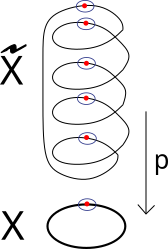
\includegraphics[scale=0.5]{./imagenes/spring.png}
  \end{figure}
  Ciertamente el intervalo \([0, 10 \pi]\) con \(0 \sim 10 \pi\) cumple
  el requisito, con el cubrimiento dado por
  \begin{align*}
    p : [0, 10 \pi] / _{(0 \sim 10\pi )} &\longrightarrow [0, 2 \pi] / _{(0 \sim 2\pi )} \\
    t &\longmapsto \mathrm t \mod 2 \pi
  \end{align*}

  Como acotacion, notar que si nuestro cubrimiento fuera \([0, 10 \pi]\)
  sin identificar los bordes y la misma función \(p\), entonces este no
  seria un cubrimiento. Esto se ve a pensar cual vecindad de \(0 \in
  [0,2\pi] / \{0 \sim 2\pi\}\) es cubierta con las propiedades. Tomando
  cualquier vecindad \(U_0\), se cumple que la pre-imagen bajo \(p\) es de
  la siguiente forma
  \[
    [0,b) \cup
    \bigcup_{k \in \{2,4,6,8\}} (k\pi - a, k\pi + b)
    \cup (10\pi - a, 10\pi]
  \]
  con los dos conjunto extremos no cumpliendo que la restricción de
  \(p\) a ellos sea un homeomorfismo local.
\end{ejemplo}
El diagrama anterior da una idea de la forma de general los espacios
cubrimientos \(\tilde X\), estos lucen como iteraciones del espacio base
\(X\). Por otro lado, sea \(x_0 \in S^1\) el punto rojo del diagrama, se
tiene la siguiente definicion auxiliar
\begin{definicion}[Fibra]
El conjunto dado por \(p^{-1} (x_0)\) es conocido como una
\emph{fibra} de \(x_0\).
\end{definicion}
\noindent Una invariante interesante es que para espacio conexos, la
cardinalidad de la fibra es la misma para todos los puntos.

\begin{teorema}
  Si \(X\) es un espacio conexo y \(p : \tilde X \to X\) es un
  cubrimiento. Si existe \(\b_1 \in X\) tal que
  \[ \text{card} \left( p^{-1} (b_1) \right) = k \]
  para alguna cantidad \(k\), entonces para todo \(b \in X\) se cumple
  que
  \[ \text{card} \left( p^{-1} (b) \right) = k \]
\end{teorema}
\begin{proof}
  Se definen dos conjuntos
  \begin{gather*}
    A := \{ b \in X \mid \text{card} \left( p^{-1} (b) \right) = k
      \} \\
    A^c := \{ b \in X \mid \text{card} \left( p^{-1} (b) \right) \neq
      k \}
  \end{gather*}
  Probaremos que ambos son abiertos. Sea \(b_1 \in A\) un elemento
  arbitrario, queremos encontrar una vecindad de este contenida en
  \(A\). Por ser \(X\) un espacio cubierto, \(b_1\) tiene una vecindad
  \(U_1\) tal que
  \[ \bigcup_{\alpha \in \Lambda} V_\alpha = p^{-1} (U_1) \]
  tal que
  \[\forall \alpha \in \Lambda, \ p \mid_{V_\alpha} : V_\alpha \to
    U_1 \text{ es un homeomorfismo} \]
  lo cual nos dice que para todo \(\alpha \in \Lambda\) existe un único
  elemento en \(V_\alpha\) que es pre-imagen de \(b_1\). Dado que la
  cardinalidad de \(p^{-1} (b_1) = k\), la cardinalidad de \(\Lambda\)
  debe de ser \(k\). Por tanto todo elemento en la pre-imagen de \(U_1\)
  tiene cardinalidad \(k\). Luego \(U_1\) es una vecindad abierta de
  \(b_1\) contenida en \(A\).

  El argumento anterior se puede hacer de igual manera para el conjunto
  \(A^c\). Por tanto, este también es un conjunto abierto. Obtenemos asi
  que \(A\) es abierto y cerrado en un espacio conexo, lo cual implica que
  este es \(X\) o \(\emptyset\). Pero como \(b_0 \in A\), se tiene que
  \(A = X\), diciendo así que todo elemento tiene la misma cardinalidad.
\end{proof}

Dado que siempre estaremos trabajando sobre espacios arco-conexos esta
propiedad siempre se tiene. Estudiemos algunos ejemplos de cubrimientos
para desarrollar intuición.

\begin{ejemplo}[Cubrimiento de toro] \label{ej:cubrimiento-toro}
  En el ejemplo \ref{ej:toro-presentacion} se trabajo con la
  presentación de toro como espacio cociente de \([0,1]^2\). Siguiendo
  la idea del ejemplo anterior, podemos obtener un cubrimiento de esta
  presentación mediante el siguiente diagrama.
  \begin{figure}[h]
    \centering 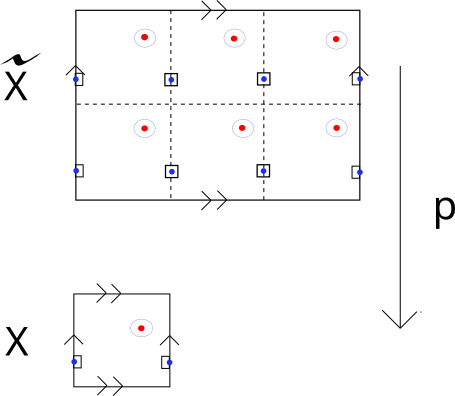
\includegraphics[scale=0.5]{./imagenes/toro-cubrimiento.png}
    \caption*{Ejemplo \ref{ej:cubrimiento-toro}: Cubrimiento del toro}
  \end{figure}
  La funcion en este caso corresponderia a
  \begin{gather*}
    \tilde X = [0,3] \times [0,2] \, / \, \{
      (x,0) \sim (x, 1), \ (0,y) \sim (1,y) \} \\
    X = [0,1] \times [0,1] \, / \, \{
      (x,0) \sim (x, 1), \ (0,y) \sim (1,y) \}
  \end{gather*}
  \begin{align*}
    p : \tilde X &\longrightarrow X \\
    (a,b) &\longmapsto \left( a \mod {1}, b \mod {1} \right)
  \end{align*}

  Aquí se muestran dos fibras de diferentes puntos iniciales. Notar que
  el punto con la vecindad rectangular esta en el borde identificado,
  por tanto su vecindad se refleja mediante esta. Esto se hereda en su
  cubrimiento que también tiene identificaciones de igual menera.
\end{ejemplo}

\begin{ejemplo}[Cubrimiento: \(\Re\) sobre \(S^1\)]
Para \(S^1\) el mapeo
\begin{align*}
  p : \Re &\longrightarrow S^1 \\
  t &\longmapsto e^{2 \pi \imath t}
\end{align*}
es claramente
sobreyectivo y continuo. Escogiendo dos abiertos ejemplares como \(U =
S^1 - \{(1,0)\}\) y \(V = S^1 - \{(-1,0)\}\), es claro que
\[
    p^{-1} (U) = \bigcup_{n \in \mathbb Z} (n, n+1)
    \qquad p^{-1} (V) = \bigcup_{n \in \mathbb Z} (n - \frac 1 2, n + \frac 1
    2 )
\]
Donde estas familias de conjuntos son disjuntos y restringidos a cada
uno se tiene la inyectividad requerida.
\end{ejemplo}

A priori el cubrimiento es independiente de los caminos que tengamos
en \(X\), queremos ver si podemos reflejar la información importante de
los caminos de \(X\) sobre \(\tilde{X}\);
\begin{figure}[h]
  \centering
  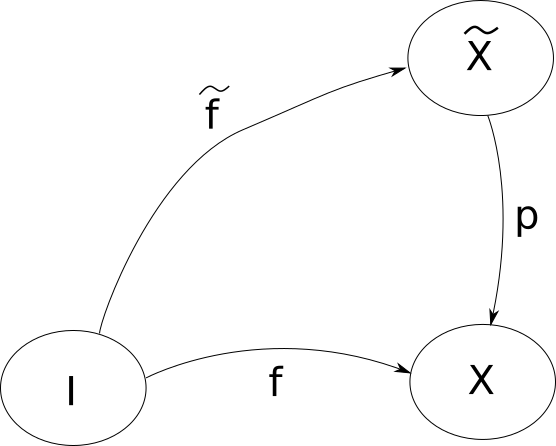
\includegraphics[scale=0.3]{./imagenes/lifting-path.png}
\end{figure}
es decir, para todo arco \(f : I \to X\), construiremos \(\tilde f : I
\to \tilde X\) el cual cumpla \(p \circ \tilde f = f \), donde \(\tilde
f\) sera nuestro representante en el espacio cubrimiento de este
camino. Veremos también que bajo ciertas hipótesis, este \(\tilde f\)
es único y refleja información homotópica. Para esto necesitamos
desarrollar algunos teoremas previos.
\begin{lema}[Número de Lebesgue] \label{lem:lebesgue-number-lema}
  Sea \(\mathcal A\) un cubrimiento del espacio métrico \((X,d)\). Si
  \(X\) es compacto, entonces existe \(\delta > 0\) tal que para todo
  subconjunto de \(X\) teniendo diámetro menor que \(\delta\), existe un
  elemento de \(\mathcal A\) conteniéndolo.
\end{lema}
\begin{proof}
  Supongamos que \(X \not \in \mathcal A\), pues si no trivialmente el
  teorema se cumple \(\forall \delta > 0\). Por compacidad de \(X\)
  existe una colección \(\{A_1 \dotsc A_n\} \subset \mathcal A\) que
  cubre a \(X\), definamos a los conjuntos \(C_i = X - A_i,\ \forall i
  \in \{1 \dotsc n\}\) y a la función \(f : X \to \Re\) definida por
  \[ f(x) := \frac 1 n \sum_{i=1}^{n} d(x, C_i) \]
  i.e. un promedio de distancias. Notemos que \(\forall x
  \in X,\ f(x) > 0\), pues para \(x \in A_i \subseteq X\), por ser
  \(A_i\) un abierto, existe \(\epsilon > 0\) tal que \(B(x,\epsilon)
  \subset A_i\) y por tanto \(d(x, C_i) \geq \epsilon\) que implica \(
  f(x) \geq \frac \epsilon n > 0\).

  Por otro lado \(f\) es una función continua. Esto por ser suma y
  ponderación sobre funciones \(d(x,C_i)\) las cuales son continuas en
  \(x\). Dado que \(f\) esta definida sobre \(X\) un espacio
  compacto, esta alcanza un mínimo; a este valor le denotaremos como
  \(\min_X f \coloneqq \delta \).

  Probaremos que este \(\delta\) cumple el requerimiento. Sea \(B
  \subset X\) subconjunto abierto de diámetro menor que \(\delta\), sea
  \(x \in B\) arbitrario. Escojamos el conjunto \(C_m\) como aquel con
  la distancia mayor a \(x\)
  \[ \forall i \in \{1 \dots n\}, \ d(x, C_m) \geq d(x, C_i) \]
  Dado que
  \[\delta \leq f(x) \leq d(x, C_m) \]
  Esto nos dice que dado \(\delta \leq d(x, C_m)\), existe una vecindad
  de al menos diámetro \(\delta\) que contiene a \(x\) en \(X - C_m = A_m\).
\end{proof}
\begin{definicion}[Levantamiento de \(f\)]
  Sea \(p : \tilde X \to X\) un mapeo. Si \(f : W \to X\) es un mapeo
  continuo, un levantamiento de \(f\) es una función \(\tilde f : W \to
  \tilde X\) tal que \(p \circ \tilde f = f\).
\end{definicion}
Ver que la definición es mucho mas general que lo que pedíamos al
diagrama. Usualmente \(W = [0,1]\) pues estudiaremos los caminos sobre
\(X\). Veremos a continuación teoremas de como se reflejan los caminos
y las homotopías en el espacio cubrimiento de \(X\).
\begin{teorema}[Levantamiento de caminos] \label{thm:lifting-theorem}
  Sea \(p : \tilde X \to X\) un cubrimiento y \(x_0 \in X\). Fijemos
  algún \(\tilde x _0 \in \tilde X\) tal que \(p(\tilde x _0) = x_0 \).
  Para cualquier camino \(f : [0,1] \to X\) que comience en \(x_0\), existe
  un único camino levantamiento \(\tilde f : [0,1] \to \tilde X\) tal que
  \(\tilde f (0) = \tilde x _0\)
\end{teorema}
\begin{proof}
  Para todo punto de \(x \in X\), existe una vecindad de este \(U_x\)
  que es cubierta (definicion \ref{def:cubierta}). Por tanto
  \[ X \subseteq \bigcup_{x \in X} U_x\]
  con \(U_x\) siendo las vecindades cubiertas para cada \(x\). De lo
  anterior, se obtiene la siguiente inclusion
  \[ [0,1] = f^{-1} \left( X \right) \subseteq f^{-1} \left( \bigcup_{x
    \in X} U_x \right) \]
  Por el Teorema \ref{lem:lebesgue-number-lema}, podemos elegir
  \(s_0,\dotsc,s_n \in [0,1]\) tal que para todo \(i \in \{0,1 \dotsc,
  n-1\}\), exista \(U_x\) tal que
  \[f \left( [s_i, s_{i+1}] \right) \subset U_x \]
  Con esto, definiremos \(\tilde f\) inductivamente.

  Primero declaremos \(\tilde f (0) = \tilde x _0\). Luego, suponiendo
  que \(\tilde f (s)\) esta definido para \(s \in [0, s_i]\), se
  define a \(\tilde f \) en \([s_i, s_{i+1}]\) de la siguiente forma.
  Dado que para algún \(x \in X\),
  \[
    f \left( [s_i, s_{i+1}] \right) \subseteq U_x \quad \land \quad
    \exists \{V_\alpha\}_{\alpha \in \Lambda},\ \bigcup_{\alpha \in \Lambda}
    V_\alpha = p^{-1} (U_x)
  \]
  debe de existir \(\alpha \in \Lambda\) tal que \(\tilde f (s_i) \in
  V_\alpha\) previamente definido; a este conjunto le denotaremos
  \(V_0\). Dado que \(p \mid_{V_0}\) es un homeomorfismo, definimos a
  \(\tilde f (s)\) en \([s_i, s_{i+1}]\) por
  \begin{equation} \label{eq:tilde-f-inductiva}
    \tilde f (s) = \left( p \mid _{V_0} \right)^{-1} \left( f(s) \right)
  \end{equation}
  El cual es continuo en \([0, s_i] \cup [s_i, s_{i+1}]\) en virtud del
  lema del pegamiento y bien definido por ser \( p \mid _{V_0} \)
  homeomorfismo.

  Para ver la unicidad, se probara inductivamente. Supongamos que existe
  otro \(\hat{f}\) levantamiento par de \(f\) que también
  comienza en \(x_0\), ie \(\hat{f} (0) = \tilde x _0 = \tilde f
  (0)\). Supongamos que
  \begin{equation}
    \label{eq:tilde-f-def-si}
    \forall s \in [0, s_i],\ \hat{f} (s) = \tilde f (s)
  \end{equation}
  Dado que \(\tilde f\) esta definida por
  \eqref{eq:tilde-f-inductiva}, \(\hat f\) debe ser
  eventualmente diferente a la definición \eqref{eq:tilde-f-inductiva},
  pero por \eqref{eq:tilde-f-def-si}
  \[\hat f (s_i) = \tilde f (s_i) \in V_0,\ \text{para algún conjunto } V_0 \]
  Como \([s_i, s_{i+1}]\) conexo y la familia \(\{V_\alpha\}\)
  es disjunta, obliga\footnote{Funciones continuas mapean conjuntos
    conexos a conexos.} a que
  \[ \hat f \left( [s_i, s_{i+1}] \right) \subset V_0 \]
  Por ser \(\hat f\) un levantamiento, este debe de cumplir la ecuación
  \begin{align*}
    \forall s \in [s_i, s_{i+1}],\quad
        &p \circ \hat f \, (s) = f(s) = p \circ \tilde f \, (s) \\
    \iff \forall s \in [s_i, s_{i+1}],\quad
        &p \left( \hat f (s) \right) =
        p \left( \left( p \mid_{V_0} \right) ^{-1} \left( f (s) \right) \right) \\
    \implies \forall s \in [s_i, s_{i+1}],\quad
        &\hat f (s) = (p \mid_{V_0})^{-1} (f (s))
  \end{align*}
  siendo esta la única posible definición, pues de haber otra,
  se tendria una contradicción en decir que \((p \mid_{V_0})\) es un
  homeomorfismo (biyectivo). Por tanto se obliga a que \( \hat f =
  \tilde f\).
\end{proof}
Mas aun, podemos no solo levantar las curvas sobre \(X\) a \(\tilde X\),
si no también preservar las homotopías de \(X\) en \(\tilde X\).
\begin{corolario}[Levantamiento homotópico] \label{thm:levantamiento-homotopico}
  Sea \(p : \tilde X \to X\) un cubrimiento tal que \(p(\tilde x _0)
  = x_0 \) para algún \(\tilde x _0 \in \tilde X\). Para cualquier
  función continua \(F : I \times I \to X\) tal que \(F(0,0) = x_0\), tiene una
  única función levantamiento continua \(\tilde F : I \times I \to
  \tilde X\) que cumpla \(\tilde F (0,0) = \tilde x_0\)
\end{corolario}
\begin{proof}
  Lo único diferente con el lema \ref{thm:lifting-theorem} es que en
  lugar de tomar \(I\) tomamos \(I \times I\) que sigue siendo compacto.
  Podemos aplicar el lema \ref{lem:lebesgue-number-lema} anterior, primero
  definiendo \(\tilde F\) en \(0 \times I\), luego en \(I \times 0\) y
  escogiendo subdivisiones de \(I \times I\)
  \[ s_0 < s_1 < \dotsc < s_m \]
  \[ t_0 < t_1 < \dotsc < t_n \]
  tales que \(F ([s_i , s_{i+1}] \times [t_j \times t_{j+1}])\) este
  contenido en un conjunto cubierto en \(X\), esto utilizando
  el lema de Lebesgue al igual que en la demostración anterior.

  Luego definimos inductivamente \(\tilde F\) sobre \([s_i, s_{i+1}]
  \times [t_j , t_{j+1}]\) siempre y cuando \(\tilde F\) ya este
  definida sobre las lineas
  \[ L := [s_i , s_{i+1}] \times \{t_j\}\]
  \[ H := \{s_i\} \times [t_j , t_{j+1}] \]
  que son los bordes inferior y izquierdos del rectángulo.

  Tomamos el conjunto \(U\) par que contiene a la imagen
  \[ F([s_i , s_{i+1}] \times [t_j , t_{j+1}]) \subseteq U \subset X \]
  Dado que son cubiertas, podemos tomar la pre-imagen de \(p\) en \(U\) como
  \[ p^{-1}(U) = \bigcup_{\alpha \in \Alpha} V_\alpha\]
  Donde la familia \(\{V_\alpha\}\) es disjunta.

  Dado que \( \{(s_i, t_j)\} = L \cap H\) y que \( (s_i , t_j) \) ya
  esta definido bajo \(\tilde F\), existe un único \(V_0 \in
  \{V_\alpha\}\) que contiene a \(F (s_i, t_j)\). Pero notando que
  \(\{V_\alpha\}\) son disjuntos y que \(L,H\) son conexos, obliga a que
  \[ \tilde F (H) \subset V_0, \quad \tilde F (L) \subset V_0 \]
  Luego podemos definir \(\tilde F\) sobre el resto de \([s_i,
    s_{i+1}] \times [t_j , t_{j+1}]\) notando que \(p \mid_{V_0}\) es
  un homeomorfismo entre \(V_0\) y \(U\) y por tanto
  \begin{equation}\label{eq:induc-homotopia}
  \forall (a,b) \in [s_i, s_{i+1}] \times [t_j , t_{j+1}],
    \ \tilde F (a,b) := p^{-1} \mid_{V_0} \left( F(a,b) \right)
  \end{equation}
  Esta cumple la regla \( F = p \circ \tilde F\) y es continua en virtud
  del lema del pegamiento. Notando finalmente que ahora los conjuntos
  \[ L := [s_i , s_{i+1}] \times \{t_{j+1}\}\]
  \[ H := \{s_{i+1}\} \times [t_j , t_{j+1}] \]
  Están definidos en \(\tilde F\) y pueden ser utilizados para seguir
  definiéndola inductivamente sobre \(I \times I\).
%fin pagina 24
\end{proof}
\begin{corolario}\label{cor:preservar-arco-hom}
  El levantamiento homotópico de una arco-homotopía sigue siendo una arco-homotopía
\end{corolario}
\begin{proof}
  Esto es consecuencia de la definición inductiva de la ecuación
  \eqref{eq:induc-homotopia}.
\end{proof}

Retrocedamos un poco para pensar que es lo que tenemos hasta el momento.
Para un cubrimiento \(p : \tilde X \to X\), siempre es valida la
construcción de la definición \ref{def:homomorfismo-inducido} de un
homomorfismo inducido \(p_* : \pi \left( \tilde X , \tilde x _0 \right)
\to \left( X , x_0 \right)\) con \(p (\tilde x_0) = x_0\). Pero a priori
esto no nos da ninguna relación entre contención entre los grupos. Pero
cuando \(p\) es un cubrimiento, tenemos que \(p_*\) es inyectiva por el
siguiente teorema.

\begin{teorema}[Inyectividad de homomorfimos inducido por cubrimientos]
  \label{thm:inyec-covering}
  Sea \(\left( \tilde X, \tilde x_0 \right), \left( X, x_0 \right)\)
  dos espacios topológicos puntuados. Si \(p : \left( \tilde X, \tilde x_0
  \right) \to \left( X, x_0 \right)\) un cubrimiento entre estos,
  entonces el homomorfismo inducido
  \[ p_* : \pi \left( \tilde X, \tilde x_0 \right) \longrightarrow \pi
    \left( X, x_0 \right)\]
  es inyectivo.
\end{teorema}
\begin{proof}
  Que el homomorfismo \(p_*\) sea inyectivo equivale a que su
  kernel sea únicamente la identidad. Para esto
mostraremos que todo elemento \([\tilde f] \in \pi
(\tilde X , \tilde x_0)\) tal que \(p_* ([\tilde f]) = [k_{x _0}]\) con \([k_{ x _0}]\)
la identidad de \(\pi (X, x_0)\), esta obligado a cumplir \([\tilde f] =
[k_{\tilde x _0}]\) donde \([k_{\tilde x _0}]\) es la identidad de \(\pi (\tilde X ,
\tilde x _0)\).

Sea \([\tilde f] \in \pi (\tilde X, \tilde x _0)\) un elemento
arbitrario tal que
\[p_* ([\tilde f]) = [p \circ \tilde f] = [k_{ x _0}]\]
Esto equivale a decir que existe una homotopía \(H\) entre \(p_* \circ
f\) y \(k_{x _0}\). Por el corolario \ref{thm:levantamiento-homotopico} podemos
levantar esta homotopía \(H\) en \((X, x_0)\) a una homotopía
levantamiento \(\tilde H\) en \((\tilde X , \tilde x _0)\). Esta es un
levantamiento homotópico, por tanto cumple la ecuaciones
\[ p \circ \tilde H = H, \quad H (t, 0) = p \circ \tilde f, \quad H (t,
  1) = k_{x _0} \]
por lo que \(\tilde H\) es una homotopía entre los levantamientos de \(p
\circ \tilde f\) y \(k_{x _0}\). Por el teorema \ref{thm:lifting-theorem},
sabemos que estos levantamientos son únicos. También sabemos por simple
calculo que
\[ p \circ k_{\tilde x _0} (t) = p \left( \tilde x_0 \right) = x_0 =
  k_{x_0} (t) ,\quad \forall t \in [0,1] \]
por lo que \(k_{\tilde x _0}\) es el levantamiento de \(k_{x_0}\).
Además de ya conocer que \(\tilde f\) es el levantamiento de \(p \circ
\tilde f\). Por tanto \(\tilde H\) es una homotopía entre \(\tilde f\) y
\(k_{\tilde x _0}\) ie
\[[\tilde f] = [k_{\tilde x_0}]\]
obteniendo así que el kernel de \(p_*\) es trivial.
\end{proof}

Hemos mostrado que para un cubrimiento \(p : (\tilde X, \tilde x _0) \to
(X , x_0)\), se tiene que
\[ \pi (\tilde X, \tilde x_0) \simeq p_* \left( \pi (\tilde X, \tilde x_0)\right) \]
donde \(p_* \left( (\tilde X, \tilde x_0) \right)\) es un subgrupo de
\(\pi (X, x_0)\). Con esto podemos revisar algunos ejemplos anteriores.
\begin{ejemplo}[Ejemplo \ref{ej:10pi} continuado]
  En el ejemplo anterior se había definido \(p : [0 , 10 \pi] /_{0 \sim
    10\pi} \to [0, 2\pi] /_{0 \sim 2\pi}\).
  \begin{figure}[h]
    \centering 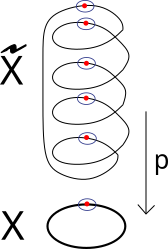
\includegraphics[scale=0.5]{./imagenes/spring.png}
  \end{figure}
  Consideremos a \(x_0 \in [0, 2\pi] /_{0 \sim 2\pi}\) un punto base. El
  homomorfimos inducido para \(p\) corresponde a la función
  \begin{align*}
    p_* : \pi \left( [0, 2\pi] /_{0 \sim 2\pi} , x_0 \right) &\longrightarrow \left( [0, 10\pi] /_{0 \sim 10\pi}, x_0 \right) \\
    [f] &\longmapsto [p \circ f]
  \end{align*}
  Según el diagrama, el claro ver que ambos grupos solo admiten una
  curva no trivial en ellos. Llamaremos
  \begin{gather*}
    [\gamma] \in \pi \left( [0, 10\pi] /_{0 \sim 10\pi}, x_0 \right),\
    \gamma (t) := 10 \pi t \\
    [\alpha] \in \pi \left( [0, 2\pi] /_{0 \sim 2\pi}, x_0 \right), \
    \alpha (t) := 2 \pi t
  \end{gather*}
  a estas. Calculando la imagen de \([\gamma]\) bajo \(p_*\) se obtienen
  las siguiente ecuaciones
  \begin{equation*}
    p_* \left( [\gamma] \right) = [p \circ \gamma]
  \end{equation*}
  donde
  \[
    p \circ \gamma (t) = 10 \pi t \mod 2 \pi = \alpha^5
  \]
  luego, reemplazando en la ecuación anterior
  \begin{equation*}
    p_* \left( [\gamma] \right) = [p \circ \gamma] = [\alpha^5] =
    [\alpha]^5
  \end{equation*}
  Dado que \(p_*\) es un homomorfismo, es claro que \(p_* \left(
  [\gamma]^n \right) = [\alpha]^{5n}\). Conociendo que \(\pi \left(
  [0,2\pi] /_{0 \sim 2\pi} , x_0 \right)\) es \((\mathbb Z, +)\) es claro
  ver que \(p_* \left( \pi \left( [0, 10\pi] , x_0 \right) \right)\) es
  \(5 \mathbb Z \) que es isomorfo (ambos tienen un unico generador) a
  \(\mathbb Z\).
\end{ejemplo}

Una pregunta ha hacerse sobre el teorema \ref{thm:inyec-covering} es si
tenemos esta implicación en sentido contrario, esto es, si todo subgrupo
de \(\pi(X, x_0)\) le corresponde un cubrimiento el cual cumpla esta
relación. La respuesta es afirmativa. La demostración no es nuestro
enfoque, pero se invita a los interesados en revisar el teorema 1.3.6 de
Hatcher \cite{Hatcher}.

Es mas claro la forma de calcular grupos fundamentales usando
cubrimientos. Si estudiamos las imágenes de distintos cubrimientos en el
espacio base, los distintos subgrupos nos darán una idea de
quien debe ser el grupo fundamental del espacio base, pues este debe de
ser compatible con todos los distintos subgrupos generados mediante
cubrimientos. Sin embargo, esta técnica no nos asegura determinar el
grupo del espacio base \(\pi (X, x_0)\) pues nos falta la
sobreyectividad. Buscar condiciones para garantizar esta propiedad es
infructuoso en termino de teoremas. Se adopta otro enfoque en general,
el de estudiar las acciones del grupo \(\pi \left( X, x_0 \right)\)
sobre la fibra \(p^{-1} \left( x_0 \right)\), el cual probaremos que
bajo condiciones sensatas sobre el cubrimiento \(p\) y el espacio
cubrimiento \(\left( \tilde X, \tilde x _0 \right)\), es isomorfo a \(\pi
(X, x_0)\). Estas condiciones están intrínsecamente relacionadas con el
cubrimiento universal

\subsubsection{Cubrimiento universal}
\begin{definicion}[Simplemente conexo]
  Un espacio topológico \(X\) es simplemente conexo si su grupo
  fundamental es trivial.
\end{definicion}
\begin{acotacion}
  Para un espacio simplemente conexo, para cualquier par de arcos
  existe una homotopía entre ellos (la composición de sus dos homotopías
  al arco identidad \(k_{x_0}\)).
\end{acotacion}
Intuitivamente estos espacios son aquellos que todos caminos cerrados
son triviales. Ejemplo de estos son los distintos \(\Re^n\) para
distintos valores de \(n\).
\begin{definicion}[Cubrimiento universal]
  Sea \(\left( X, x_0 \right)\) un espacio topológico puntuado. Un
  cubrimiento \(p : \left( \tilde X , \tilde x _0 \right) \to \left( X ,
    x _0 \right)\) es llamado cubrimiento universal de \( \left(
    X , x _0 \right)\) si \(\left( \tilde X , \tilde x _0
  \right)\) es simplemente conexo.
\end{definicion}
El estudio de los cubrimientos universales esta relacionado con el
comportamiento de una funcion conocida como el levantamiento derivado.
\begin{definicion}[Levantamiento derivado] \label{def:levantamiento-derivado}
  Sea \(p : \tilde X \to X\) un cubrimiento y sea \(x_0 \in X\).
  Escojamos \(\tilde x _0 \in \tilde X\) tal que \(p(\tilde x _0) =
  x_0\). Dado un elemento \([f] \in \pi (X, x_0)\), sea \(\tilde f\) el
  levantamiento (único) de \(f\) a un camino en \(\tilde X\) que
  comienza en \(\tilde x _0\). Se define una función
  \begin{align*}
    \phi_{\tilde x_0} : \pi (X, x_0) &\longrightarrow p^{-1} (x_0) \\
    [f] &\longmapsto \tilde f (1)
  \end{align*}
  y denominamos a \(\phi_{\tilde x_0}\) como el \textbf{correspondiente
  levantamiento derivado}\footnote{Corresponding lifting path} del
  cubrimiento \(p\). Cuando no haya incertidumbre se denotara a este
  simplemente \(\phi\).
\end{definicion}
\begin{acotacion} \label{aco:indep-phi}
  Este mapeo no depende del representante de clase \([f] \in \pi \left(
    X, x_0 \right)\). Para ver esto, notar que tomando a \(f_1 \in [f]
  ,\ f_1 \neq f\) estos están relacionados por una arco-homotopía
  \(H\). Por el teorema \ref{thm:levantamiento-homotopico} de
  levantamiento homotópico, existe una homotopía \(\tilde H\) la cual me
  relaciona los levantamientos \(\tilde f_1 , \tilde f\) de \(f_1 , f\)
  respectivamente. Pero dado el corolario \ref{cor:preservar-arco-hom},
  la homotopía \(\tilde H\) es una arco-homotopía y por tanto
  \[ \tilde f (1) = \tilde H (1, 1) = \tilde H (1, t) = \tilde H (1, 0)
    = f_1 (1) ,\ \forall t \in \{0 \dotsc 1\} \]
  lo que implica que
  \[ \phi ([f]) = \phi ([f_1])\]
\end{acotacion}

Al estudiar los caminos en el espacio base \(\left(X, x_0 \right)\)
cuando estos son levantados al espacio cubrimiento \((\tilde X ,
\tilde x _0 )\), es posible que se transformen caminos con el mismo
punto inicial y final a caminos donde esto no es necesario. Es decir es
posible que ``desenrolle'' los caminos al levantarse. Sin embargo para
cumplir la propiedad de los levantamiento, el punto final de este tiene
que pertenecer al conjunto \(p^{-1} \left( \{x_0\} \right)\), es decir
la fibra de \(x_0\). De hecho podemos enfocarnos puramente en el punto
al que permuta el punto final y podríamos determinar totalmente al arco
en la base al que corresponde cuando el cubrimiento sea universal. Esto
se vera en la siguiente teorema.
\begin{teorema} \label{thm:phi-bijec}
  Sea \(p : \tilde X \to X\) un cubrimiento tal que \(p (\tilde x _0) =
  x_0\). Si \(\tilde X\) es arco-conexo entonces el correspondiente
  levantamiento \(\phi : \pi (X, x _0) \to p^{-1} (x_0)\) basado en
  \(\tilde x_0\) es sobreyectivo. Mas aun, si \(\tilde X\) es
  simplemente conexo, este es biyectivo.
\end{teorema}
\begin{proof}
  Demostración estándar de sobreyectividad en caso de ser \(\tilde X\)
  arco-conexo. Para \(\tilde x _1 \in p^{-1} (x_0)\) arbitrario, existe
  \(\tilde f\) camino entre \(\tilde x _0 \) a \(\tilde x _1\) por
  arco-conexidad. Definimos \(f := p \circ \tilde f\), el cual es un
  camino \(f : I \to X\) que cumple \(\phi ([f]) = \tilde x _1\) por
  definición.

  En caso de ser \(\tilde X\) simplemente-conexo, veremos solo la
  inyectividad. Sean \([f],[g] \in \pi (X, x_0)\) tales que \(\phi([f])
  = \phi([g])\), mostraremos que \([f] = [g]\). Sean \(\tilde f, \tilde
  g : I \to \tilde X\) los levantamientos respectivos que comienzan en
  \(\tilde x _0\). Dado que \(\phi([f]) = \tilde f (1) = \tilde g (1) =
  \phi([g])\) y la simple-conexidad de \(\tilde X\), existe \(\tilde F :
  I \times I \to \tilde X\) homotopía de \(\tilde f, \tilde g\) que
  cumple
  \[ \tilde F (0, t) = \tilde x_0, \quad \tilde F (1 , t) = \tilde f
    (1) = \tilde g (1)
  \]
  Luego \(p \circ \tilde F : I \times I \to X \) es una homotopía entre
  \(f, g\), por tanto \([f] = [g]\)
\end{proof}
% \begin{acotacion}
%   Esta versión del teorema es la mas útil desde el punto de vista del
%   calculo pero no la mas general. Ese enunciado corresponde a estudiar las
%   acciones del grupo \(\pi (X , x_0)\) sobre la fibra. La biyeccion se
%   obtiene de pedir que el cubrimiento sea \emph{regular}, requerimiento
%   que se cumple con pedir simple-conexidad de \((X, x_0)\). Para ver el
%   teorema completo se dirige \cite{Hatcher}[pag. 69]
% \end{acotacion}
Este teorema nos permitirá enfocarnos puramente en la fibra \(p ^{-1}
(x_0)\) para estudiar el grupo fundamental de \((X, x_0)\). Por otro
lado, podemos definir un nuevo grupo el cual va a actuar (en sentido de
grupos) sobre esta fibra al cual denotaremos como grupo de
transformaciones de \emph{deck}\footnote{En español seria transformaciones de
  cartas, pero asi podemos utilizar un nombre usual de \cite{Hatcher}}.
\begin{definicion}[Grupo de transformaciones de \emph{deck}]\label{def:deck}
  Para un cubrimiento \(p : \tilde X \to X\), los isomorfismos \(g : \tilde
  X \to \tilde X\) tales que cumplan
  \[ p \circ g = p \]
  son transformaciones de \emph{deck}. El grupo \(G (\tilde X)\) formado
  por estos isomorfismos, la composición como operación forman el grupo
  de transformaciones de \emph{deck} con la función identidad como
  identidad de grupo.
\end{definicion}
Para ver la relación del grupo \(G(\tilde X)\) con la fibra \(p^{-1}
(x_0)\) es necesario generalizar algunos resultados de levantamientos de
caminos (teoremas \ref{thm:lifting-theorem},
\ref{thm:levantamiento-homotopico})

\begin{teorema}\label{thm:lifting-theorem-general}
  Sea \(p : (\tilde X , \tilde x_0) \to ( X , x _0 )\) un cubrimiento y
  \(f : (Y , y_0) \to ( X , x _0 )\) una funcion continua con \(Y\)
  arco-conexo y localmente arco-conexo. Entonces un levantamiento
  \(\tilde f : (Y , y_0) \to (\tilde X, \tilde x _0)\) de \(f\) existe
  si y solo si
  \[ f_* \left( \pi (Y, y_0) \right) \subseteq p_* \left( \pi ( \tilde X
      , \tilde x_0 ) \right) \]
  \begin{center}
    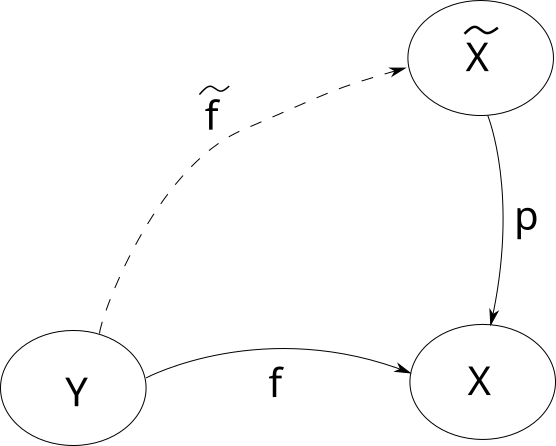
\includegraphics[scale=0.3]{./imagenes/lifting-path-gen.png}
  \end{center}
\end{teorema}
Que un espacio \(Y\) sea localmente arco-conexo equivale a pedir que
para todo punto \(y \in Y\) y cualquier vecindad \(U_y \subset Y\) de
este, posee una sub-vecindad \(V \subseteq U_y\) la cual es arco-conexa.
Procedemos a la demostración.
\begin{proof}
  Se procede en la dirección \((\Rightarrow)\). Por simple definición,
  es fácil ver que \(f_* = p_* \circ \tilde f _*\) lo cual implica
  directamente el resultado.

  Ahora mostraremos la dirección \((\Leftarrow)\). Sea \(y \in Y\) un
  punto arbitrario para el cual dada la arco-conexidad de \(Y\) existe
  un camino \(\gamma\) en \(Y\) tal que
  \[\gamma (0) = y_0,\ \gamma (1) = y\]
  Con este podemos definir un camino \(f \circ \gamma\) en \(X\) el cual
  cumple con comenzar en \(x_0\). Por el teorema
  \ref{thm:lifting-theorem}, este ultimo camino tiene un (único)
  levantamiento \(\widetilde {f \circ \gamma}\) tal que \(\widetilde{f
  \circ \gamma} (0) = y_0 \). Mediante este, definimos una función
  \(\tilde f : (Y, y_0) \to (\tilde X , \tilde x_0)\) por la ecuación
  \begin{equation} \label{def:f-tilda}
    \tilde f (y) := \widetilde{f \circ \gamma} \, (1)
  \end{equation}
  Si probamos que \(\tilde f\) esta bien definido y es continua
  obtendremos que es el levantamiento buscado.

  % sacado de ../pdf-informacion/cls15--lifting.properties.pdf
  Mostrar que esta bien definido equivale a mostrar que \(\tilde f\) es
  independiente del camino \(\gamma\) entre \(y_0 \to y\). Tomemos otro
  camino \(\delta\) entre \(y_0 \to y\) y fijemos el camino \(g\)
  \[ g = f \circ \left( \delta * \overline{\gamma} \right)
    = (f \circ \delta) * \overline{(f \circ \gamma)} \]
  Es claro que \(g\) es un camino cerrado de \(x_0 \to x_0\) en \(X\)
  y por construcción e hipótesis cumple la inclusión
  \[ [g] \in f_* \left( \pi (Y, y_0) \right) \subseteq p_* \left( \pi
      (\tilde X, \tilde x_0) \right)\]
  Sea \(\tilde g\) el levantamiento de \(g\) tal que \(\tilde g
  (0) = \tilde x_0\). Dado que \([g] \in p_* \left( \pi (\tilde X
    ,\tilde x_0) \right)\) este levantamiento esta obligado ha ser un
  camino cerrado de \(\tilde x_0 \to \tilde x_0\). Por ultimo, notamos
  que por construcción
  \[ \forall t \in [0, \frac 1 2],\ g(t) = f \circ \delta (2 t) \]
  lo que implica por unicidad del levantamiento en \(\tilde x_0\) que la
  primera mitad del levantamiento \(\tilde g\) corresponde a
  \(\widetilde{f \circ \delta}\). De igual manera, considerando el
  camino inverso \(\overline{g}\) también de \(x_0 \to x_0\), este
  cumple la ecuación
  \[ \forall t \in [0, \frac 1 2],\ \overline{g}(t) = f \circ \gamma (2
    t) \]
  y otra vez por unicidad del levantamiento en \(x_0\), se cumple que la
  primera mitad de su levantamiento \(\widetilde{\overline{g}}\)
  corresponde a \(\widetilde{f \circ \gamma}\). Dado que
  \[ \forall t \in [\frac 1 2 , 1],\ g(t) = \overline{g} (1 - t) \]
  se tiene que \(\overline{(\widetilde{f \circ \gamma})}\) corresponde a la
  segunda mitad de \(\tilde g\). En resumen se cumple que \(g\) cumple
  la ecuación
  \[ \tilde g = \widetilde{f \circ \delta} * \overline{(\widetilde{f
  \circ \gamma})} \] y dado que \(\tilde g\) esta bien definido, se debe
  cumplir que
  \[ \widetilde{f \circ \delta} (1) = \widetilde{f \circ \gamma} (1) \]
  mostrando la independencia de la función \(\tilde f\).

  Por ultimo probaremos la continuidad de \(\tilde f\) en \(y\). Sea \(U
  \subseteq X\) una vecindad de \(f (y)\). Por definición de cubrimiento,
  existe al menos un conjunto \(\tilde U \subseteq \tilde X\) tal que
  \[p \mid_{\tilde U} : \tilde U \to U\]
  es un homeomorfismo. Por otro lado, dada la continuidad de \(f\) y
  por ser \(Y\) localmente arco-conexo se puede elegir una vecindad \(V
  \subseteq Y\) arco-conexa de \(y \in Y\) tal que \(f (V) \subset U\).
  Para todo \(y' \in V\), consideremos los caminos cerrados en \(X\)
  \[ \gamma * \eta * \overline{\eta} * \overline{\gamma} \]
  con \(\gamma\) un camino entre \(y_0 \to y\) y \(\eta\) un camino
  entre \(y \to y'\). Al ver la imagen de este camino bajo \(f\) esta
  corresponde al camino
  \[ (f \circ \gamma) * (f \circ \eta) * (f \circ \overline{\eta}) * (f
    \circ \overline{\gamma}) \]
  en \(X\). Por hipótesis este camino puede ser levantado a
  \(\tilde X\) al camino
  \[ \widetilde{f \circ \gamma} * \widetilde{f \circ \eta} *
    \widetilde{f \circ \overline{\eta}} * \widetilde{f \circ
    \overline{\gamma}} \]
  En particular es claro que por ser \(p \mid_U\) un homeomorfismo y \(f
  (V) \subset U\) se tiene que
  \[ \widetilde{f \circ \eta} = p^{-1} \circ f \circ \eta \]
  por la ecuación de levantamiento. Lo que al juntarse con la ecuación
  \eqref{def:f-tilda} implica que \(\tilde f (V) \subseteq \tilde U\) y en
  particular \( \tilde f \mid _{V} = p^{-1} \circ f \) lo cual es
  composición de una función continua con un homeomorfismo y por tanto
  continua en \(y\).
\end{proof}

\begin{teorema}[Unicidad levantamiento]\label{thm:uniq-general}
  Dado un cubrimiento \(p : \tilde X \to X\) y un mapeo \(f : Y \to X\),
  si dos levantamientos \(\tilde f _1 , \tilde f _2 : Y \to \tilde X\)
  de \(f\) concuerdan en un punto de \(Y\) y \(Y\) es conexo, entonces
  \(\tilde f _1 , \tilde f _2\) concuerdan en todo \(Y\).
\end{teorema}
\begin{proof}
  Para un punto arbitrario \(y \in Y\), existe una vecindad \(U \subset
  X\) la cual es cubierta por \(p\) de manera que se cumple la
  ecuación
  \[ \bigcup_{\alpha} \tilde U_\alpha = p^{-1} \left( U \right)\]
  Con \(\tilde U _\alpha\) disjuntos y que al restringir \(p\) en ellos
  se tiene un homeomorfismo. En particular denotemos \(\tilde U
  _1 , \tilde U _2\) a los conjuntos tales que
  \[ \tilde f _1 ( y ) \in \tilde U _1,\ \tilde f _2 ( y ) \in \tilde U
    _2 \]
  Por continuidad de \(\tilde f_1, \tilde f_2 \), fijamos una vecindad
  de \(y\) por
  \[ N := \tilde f _1 ^{-1} (\tilde U _1) \cap \tilde f _2 ^{-1} (\tilde
    U _2) \]
  la cual cumple trivialmente que
  \[ \tilde f_1 (N) \subseteq \tilde U _1,\ \tilde f_2 (N) \subseteq
    \tilde U _2 \]
  Tomaremos casos. Si \(\tilde f _1 (y) \neq \tilde f _2 (y)\) implica
  que \(\tilde U _1 \neq \tilde U _2\) pues de ser el mismo conjunto, se
  tendría una contracción con la inyectividad de \(p\) al ser
  restringido a este pues se debe cumplir que \( p \circ \tilde f _1 (y)
  = p \circ \tilde f _2 (y)\). Dado que \(\tilde U_1 \neq \tilde U _ 2\)
  son disjuntos, se tiene que \(\tilde f_1 \neq \tilde f_2 \) en la
  vecindad \(N\). Por otro lado, si \(\tilde f _1 (y) = \tilde f _2
  (y)\) por el mismo argumento se debe cumplir que \(\tilde U _1 = \tilde
  U _2\) y por tanto \(\tilde f _1 = \tilde f _2\) en \(N\).

  Definamos un conjunto auxiliar
  \[ K := \{ y \in Y \mid \tilde f_1 (y) = \tilde f_2 (y) \} \]
  Por lo mostrado anteriormente, para todo punto \(y \in K\) existe una
  vecindad \(N\) totalmente contenida en \(K\). De igual manera si
  consideramos \(K^c\), también existe una vecindad \(N\) totalmente
  contenida en \(K^c\). Luego \(K\) es abierto y cerrado al mismo tiempo
  en \(Y\) un espacio conexo, lo cual obliga a que este sea \(Y\) o
  \(\emptyset\). Pero dada la hipotesis de que existe un punto donde los
  levantamientos coinciden, \(K\) no puede ser vacio y por tanto es el
  espacio total \(Y\).
\end{proof}

\begin{teorema}\label{thm:exists-isomor}
  Si \(X\) es un espacio arco-conexo, localmente arco-conexo, entonces
  dos cubrimientos \(p_1 : \tilde X _1 \to X\) y \(p_2 : \tilde X _2 \to
  X\) son isomorficos via un isomorfismo \(f : \tilde X_1 \to \tilde
  X_2\) tomando un punto base \(\tilde x_1 \in p_1^{-1} (x_0)\) a un
  punto base \(\tilde x_2 \in p_2^{-1} (x_0)\) si y solo si
  \[ p_{1,*} \left( \pi (\tilde X _1, \tilde x _1) \right) = p_{2,*}
    \left( \pi (\tilde X _2, \tilde x _2) \right) \]
\end{teorema}
\begin{proof}
  Se inicia en la direccion \(\Rightarrow\). Un isomorfismo de cubrimientos
  \(f : (\tilde X , \tilde x _1) \to (\tilde X _2, \tilde x _2)\) debe
  cumplir las ecuaciones
  \[ p_1 = p_2 \circ f,\quad p_2 = p_1 \circ f^{-1} \]
  siendo estas ecuaciones consecuencia de preservar que el espacio de
  llegada sea un cubrimiento. De la primera ecuacion se obtiene que
  \[ p_{1,*} = \left( p_2 \circ f \right)_* \]
  que por definicion al ser aplicadas a \([\gamma] \in \pi (\tilde X_1,
  \tilde x_1)\)
  \begin{equation*}
      p_{1,*} \left( [\gamma] \right) = [p_1 \circ \gamma] = [p_2 \circ
      f \circ \gamma ] = p_{2,*} \left( [f \circ \gamma] \right)
  \end{equation*}
  lo que junto la bijectividad de \(f\) implican el resultado.

  Para la direccion \(\Leftarrow\), supongamos que \(p_{1,*} (\pi
  (\tilde X _1 , \tilde x _1)) = p_{2,*} (\pi
  (\tilde X _2 , \tilde x _2))\). Por el teorema
  \ref{thm:lifting-theorem-general} de levantamiento, se puede obtener
  unos levantamientos
  \begin{gather*}
    \tilde p _1 : (\tilde X _1 , \tilde x _1) \to (\tilde X_2 , \tilde
    x_2), \ p_2 \circ \tilde p_1 = p_1 \\
    \tilde p _2 : (\tilde X _2 , \tilde x _2) \to (\tilde X_1 , \tilde
    x_1), \ p_1 \circ \tilde p_2 = p_2
  \end{gather*}
  De lo cual reemplazando adecuadamente podemos obtener
  \begin{gather*}
    p_2 \circ \tilde p _1 \circ \tilde p _2 = p_2 \\
    p_1 \circ \tilde p _2 \circ \tilde p _1 = p_1
  \end{gather*}
  lo cual debido a que estos mapeos fijan los puntos bases respectivos,
  podemos aplicar el teorema \ref{thm:uniq-general} de unicidad
  del levantamiento obteniendo asi que
  \[ \tilde p_1 \circ \tilde p_2 = \text{Id}, \quad \tilde p_2 \circ
    \tilde p_1 = \text{Id} \]
  Por tanto \(\tilde p_1 , \tilde p_2\) son isomorfismos inversos
  (Corolario \ref{thm:comp-identidad}).
\end{proof}

Ahora nos enfocaremos en un caso especifico, cuando nuestro cubrimiento
es universal. Sea \(p : \tilde X \to X,\ \tilde X\) un
cubrimiento universal de \(X\). Sea \(x_0 \in X\) un punto base. Es
claro que dado que el los grupos fundamentales de \(\tilde X\) son
triviales independientes del punto base de \(\tilde X\), ie para todo
\(\tilde x_1, \tilde x_2 \in p^{-1} (x_0)\)
\begin{equation*}
  \pi \left( \tilde X , \tilde x_1 \right) = \{[k_{\tilde x_1}]\},\quad
  \pi \left( \tilde X , \tilde x_2 \right) = \{ [k_{\tilde x_2}]\}
\end{equation*}
por tanto
\begin{equation} \label{hip:lifting}
  p_* \left( \pi \left( \tilde X , \tilde x_1 \right) \right) =
  \{k_{x_0}\} = p_* \left( \pi \left( \tilde X , \tilde x_2 \right)
  \right),\ \forall \tilde x_1 , \tilde x_2 \in \tilde X
\end{equation}
Por tanto, para cualquier curva \([\gamma] \in \pi (X , x_0)\), su
representante \(\gamma\) posee un único levantamiento a \((\tilde X,
\tilde x_1)\) que denotaremos por \(\tilde \gamma\). Este debe cumplir
con las ecuaciones
\[ \tilde \gamma \, (0) = \tilde x_1, \quad \tilde \gamma \, (1) =
  \tilde x_2 = \phi ([\gamma]) \]
para algún \(\tilde x_2 \in p^{-1} (x_0)\). La ecuación
\eqref{hip:lifting} aplicada a estos \(\tilde x_1, \tilde x_2,\) nos
permite aplicar el teorema \ref{thm:exists-isomor} que nos da un
isomorfismo de cubrimientos
\[\varphi : (\tilde X , \tilde x_1) \to (\tilde X , \tilde x_2 ) \]
el cual cumple la ecuación \(p \circ \varphi = p\) y por tanto es una
transformación de \emph{deck} en el sentido de la definición
\ref{def:deck}. Mas aun, \(\varphi\) es el unico isomorfismo posible
entre \((\tilde X , \tilde x_1) \to (\tilde X , \tilde x_2 )\) pues de
haber otro, tendria que compartir el punto \(\tilde x_2\) con
\(\varphi\) y iria en contra el Teorema \ref{thm:uniq-general} de
unicidad del levantamiento.

La relación anterior entre \([\gamma]\) y \(\varphi\) es asi funcional.
Por tanto podemos definir una función
\begin{align}
  L : \pi (X, x_0) &\longrightarrow G (\tilde X) \label{def:L} \\
  [\gamma] &\longmapsto \varphi \nonumber
\end{align}
cuando \(\tilde X\) es universal. Mas aun, podemos notar que dada la
biyeccion \(\phi\) estudiada en el teorema \ref{thm:phi-bijec} nos basta
saber a donde se envía un solo punto en \(\tilde X\) para determinar la
transformación de \emph{deck}.

Ahora podemos probar el isomorfismo entre \(G (\tilde X)\) e \(\pi (X,
x_0)\) cuando \(\tilde X\) es simplemente conexo.

\begin{teorema}
  Sea \(p : (\tilde X, \tilde x_0) \to (X , x_0) \) un cubrimiento
  universal de un espacio \(X\) arco-conexo, localmente arco-conexo.
  Entonces \(G (\tilde X)\) es isomorfo a \(\pi (X, x_0)\).
\end{teorema}
\begin{proof}
  La idea de la demostración sera el primer teorema del isomorfismo para
  grupos. Sea \(L\) la función definida en la ecuación \eqref{def:L} por
  \(L : \pi (X, x_0) \to G ( \tilde X)\), la cual es funcion por la simple
  conexidad de \(\tilde X\). Hemos de probar que este es un homomorfismo.
  Sean \([\gamma],[\gamma'] \in \pi (X , x_0)\) dos curvas arbitrarias.
  Sean \(\tilde \gamma , \tilde{\gamma '}\) los levantamientos respectivos
  de los representantes de clases, los cuales cumplen las siguientes
  ecuaciones
  \begin{gather*}
    \widetilde \gamma \, (0) = \widetilde x_0,\ \widetilde \gamma \, (1)
      = \widetilde x _1 \\
    \widetilde {\gamma '} \, (0) = \widetilde x_0,\ \widetilde {\gamma
      '} \, (1) = \widetilde x _2
  \end{gather*}
  con \(\tilde x_1 , \tilde x_2 \in p^{-1} (x_0)\). Sean
  \begin{gather*}
    L \left( [\gamma] \right) = \tau : (\tilde X , \tilde x_0) \to
    (\tilde X, \tilde x_1) \\
    L \left( [\gamma'] \right) = \tau' : (\tilde X , \tilde x_0) \to
    (\tilde X, \tilde x_2)
  \end{gather*}
  Véase que la curva \(\gamma * \gamma '\) posee como levantamiento a
  \begin{equation} \label{eq:levan-comp}
    \tilde \gamma * \tau \left( \widetilde{\gamma '} \right)
  \end{equation}
  pues \eqref{eq:levan-comp} es igual a \(\gamma * \gamma '\) al ser
  pre-compuesta por \(p\) y el levantamiento es único por el teorema
  \ref{thm:uniq-general} de unicidad del levantamiento. El camino
  \eqref{eq:levan-comp} sigue el la siguiente trayectoria (a grandes
  rasgos)
  \[ \tilde \gamma \, (0) = \tilde x_0 \longrightarrow \tilde \gamma (1) = \tilde x
      _1 = \tau \left( \tilde x_0 \right) \longrightarrow \tau \left( \tilde x_2
      \right) = \tau \left( \tau' ( \tilde x _0 ) \right)
  \]
  Por tanto se debe cumplir que la transformación de deck asociada a
  \([\gamma * \gamma']\) debe ser de la siguiente forma
  \[ L \left( [\gamma * \gamma'] \right) = \hat \tau : (\tilde X, \tilde
    x _0) \to (\tilde X , \tau \circ \tau' \, (\tilde x_0)) \]
  Por otro lado, la siguiente transformación de deck
  \[ \tau \circ \tau : (\tilde X, \tilde x _0) \to (\tilde X , \tau
    \circ \tau' \, (\tilde x_0))
  \]
  también envía al punto \(\tilde x_0\) a \(\tau \circ \tau' \, (\tilde
  x_0)\) , puesto que las transformaciones de \emph{deck} son
  levantamientos (demostración teorema \ref{thm:exists-isomor}) y que la
  composición de levantamientos es un levantamiento podemos aplicar el
  teorema \ref{thm:uniq-general} de unicidad de los levantamientos para
  concluir que
  \[ L \left( [\gamma * \gamma'] \right) = L \left( [\gamma] \right)
    \circ L \left( [\gamma'] \right)\]
  Mostrando así que es un homomorfismo.
  % \[ L \left( [p \circ \tilde \gamma] \right) = \tau \]

  Para mostrar la sobreyectividad de \(L\), es claro que cualquier
  \(\tau \in G (\tilde X)\) es de la forma
  \[ \tau : (\tilde X, \tilde x_0) \to (\tilde X, \tilde x_1) \]
  con \(\tilde x_0, \tilde x_1 \in p^{-1} (x_0)\). Como \(\tilde X\) es
  simplemente conexo, por el teorema \ref{thm:phi-bijec} se tiene que la
  función
  \[\phi_{\tilde x_0} : \pi (X, x_0) \to p^{-1} (x_0) \subseteq \tilde
    X \]
  de la definición \ref{def:levantamiento-derivado} es
  biyectiva. Por tanto \(\phi_{\tilde x_0}^{-1} (\tilde x_1) \in \pi (X,
  x_0)\) y es tal que
  \[ L \left( \phi^{-1} (\tilde x_1) \right) = \tau \]
  por construcción de \(L\) dada por la ecuación \eqref{def:L}.

  Mostraremos que \(L\) es inyectiva. Esto equivale a mostrar que su
  núcleo es trivial. Sea \([\gamma] \in \pi (X , x_0)\) un arco
  arbitrario tal que
  \begin{equation} \label{eq:L-in}
    L \left( [\gamma] \right) = Id : (\tilde X , \tilde x_0) \to
      (\tilde X, \tilde x_0)
  \end{equation}
  Mostraremos que \([\gamma] = [k_{x_0}]\) la identidad. Es claro por
  simple calculo que se tiene la ecuación
  \[ \phi \left( [k_{x_0}] \right) = \tilde x _0 \]
  Dada la ecuación \eqref{eq:L-in}, también se tiene que
  \[ \phi \left( [\gamma] \right) = \tilde x_0 \]
  Por la inyectividad de \(\phi\) cuando \(\tilde X\) es
  simplemente-conexo, esto obliga a que \([k_{x_0}] = [\gamma]\).
  Mostrando así que \(L\) es un isomorfismo.
\end{proof}

Con el isomorfismo mostrado podemos empezar a calcular. Usualmente uno
no plantea el grupo \(G (\tilde X)\) totalmente al encontrar un
cubrimiento universal de un espacio, si no mas bien estudia directamente
las acciones sobre la fibra \(p^{-1} (x_0)\) por la función
\(\phi\) de la definición \ref{def:levantamiento-derivado} y utiliza una
``decision informada'' para dotarle estructura de grupo. Para ver el
marco de trabajo, estudiaremos el grupo fundamental de \(S^1\) como
ejemplo. Utilizando los teoremas anteriores para proponer un
cubrimiento tal que \(\tilde X\) sea simplemente conexo y que pueda
preservar la estructura de grupo para ser estudiado bajo ese lente.
\begin{teorema} \label{thm:grupo-S1}
  \(\forall x_0 \in S^1,\ \pi (S^1,x_0)\) es isomorfo a \((\mathbb Z, +)\)
\end{teorema}
\begin{proof}
  Dado que \(S^1\) es arco-conexo, basta probar que este teorema es
  cierto para algún \(x_0\) en \(S^1\). Sea \(p : \mathbb R \to S^1,\
  p(t) := (\cos 2 \pi t, \sin 2 \pi t)\) el cual es fue visto anteriormente
  que es un cubrimiento . Sea \(\tilde x _0 = 0\) y \( p(\tilde x _0) =
  (1,0) =: x_0 \in S^1\). Por ser \(\mathbb R\) simplemente conexo, se
  tiene que el levantamiento correspondiente \(\phi : \pi (S^1, x_0) \to
  p^{-1} (x_0)\) es biyectivo, donde
  \[ p^{-1} (1,0) = \{t \in \mathbb R \mid (\cos 2 \pi t, \sin 2 \pi t)
    = (1, 0) \} = \mathbb Z \]
  Notamos además que de sobre todo \(\mathbb Z\) existe únicamente el
  grupo bajo la adición, este sera nuestro grupo de partida.

  Para probar que es homomorfismo, se toman \([f], [g] \in \pi
  (S^1, x_0)\) arbitrarios y \(\tilde f, \tilde g\) sus correspondientes
  levantamientos tales que \(n := \tilde f (1) = \phi ([f]),\ m :=
  \tilde g (1) = \phi ([g])\). Ahora queremos encontrar quien es el
  levantamiento de \([f] * [g]\), para esto se define el camino
  \begin{align*}
    \tilde{\tilde g} : I &\longrightarrow \mathbb R \\
    s &\longmapsto n + \tilde g (s)
  \end{align*}
  Puesto que \(p(n + x) = p(x)\) por periodicidad, se cumple que
  \[ p \circ \tilde{\tilde g} (x) = p (n + \tilde g (x)) = p (\tilde g
    (x)) = g (x) \]
  Por tanto \(\tilde{\tilde g}\) es el levantamiento de \(g\) para
  \(\tilde x_0 = n\) (en vez de \(\tilde x_0 = 0\)). Luego el producto
  \(\tilde f * \tilde{\tilde g}\) esta bien definido pues \(\tilde f (1)
  = n = \tilde{\tilde g} (0)\) y se afirma que este es el levantamiento
  de \(f * g\) pues por calculo
  \[ p \circ (\tilde f * \tilde{\tilde g}) =
     ((p \circ \tilde f) * (p \circ \tilde{\tilde g})) =
     (f * g)
  \]
  Por ultimo calculamos
  \[ \phi ([f] * [g]) = \tilde{\tilde g} (1) = n + m = \phi ([f]) + \phi
  ([g]) \]
  Por lo que \(\phi\) es un homomorfismo de grupos.
\end{proof}

El ejemplo anterior muestra a lo que nos referíamos con ``decisión
informada'' pues dotarle de estructura aditiva a \(\mathbb Z\) es algo
natural de intentar. También puede darse el caso que dada la
clasificación de grupos finitos, exista un único grupo de determinada
cardinalidad lo cual guié nuestra elección como en el siguiente ejemplo

\begin{ejemplo}[Grupo fundamental plano proyectivo]
  \(\mathbb R P^2\) puede verse como un espacio cociente de la esfera
  \(S^2\)  en \(\Re^3\) mediante la siguiente relación
  \[ \vec x \sim - \vec x \]
  Por tanto, para todo \(x_0 \in \mathbb S^2\) existe el mapeo cociente
  \[ p : (S^2, x_0) \longrightarrow (\mathbb R P^2, [x_0]) \]
  el cual sera nuestro mapeo cubrimiento.

  Cabe notar que el espacio \((S^2, x_0)\) es simplemente conexo. Esto puede
  verse tomando un camino cerrado de \(x_0\) contenido en \(S^2\)
  arbitrario, el cual se expresara en coordenadas esféricas
  \[ \gamma (t) := (1 , \theta (t) , \psi(t) )\]
  Se denota al punto \(x_0 = (1, \theta_0, \psi_0)\) en estas
  coordenadas. Luego existe la homotopía
  \[ H (t, \lambda) := (1, \lambda \theta_0 + (1-\lambda) \theta(t),
    \lambda \psi_0 + (1-\lambda) \psi(t))\]
  entre \(\gamma\) y el camino constante \(k_{x_0}\). Luego \(S^2\) es
  un cubrimiento universal de \(\mathbb R P^2\).

  Estudiando la fibra \(p^{-1} (\{[x_0]\})\) se ve esta tiene
  cardinalidad \(2\).
  \[ p^{-1} (\{[x_0]\}) = \{ x_0 , - x_0 \} \]
  Dado que \(S^2\) es un cubrimiento universal, la función
  \[ \phi : \pi ( \mathbb R P^2 , [x_0]) \longrightarrow p^{-1}
    ([x_0])\]
  es biyectiva y por tanto la cardinalidad de grupo de \(\pi ( \mathbb R
  P^2, [x_0])\) es \(2\). Dado que existe un único grupo con \(2\)
  elementos, obtenemos que \(\pi ( \mathbb R P^2, [x_0])\) es isomorfo a
  \(\mathbb Z_2\).
\end{ejemplo}

El ejemplo anterior se puede generalizar notando que \(S^n\) cubre
universalmente a \(\mathbb R P^n\) aunque la estructura de grupo dada
para distintas cardinalidades no es única. Sin embargo hay una cantidad
finitas de alternativas a probar para cada cardinalidad.

% TODO: otro ejemplo cabron de cubrimiento, posiblemente eliminando el
% resto de esta seccion.
% TODO: revisar los teoremas de la seccion de cubrimiento universal
% (retrabajarlos)
% TODO: agregar posiblemente diagramas
% TODO: agregar intuicion categorica (posiblemente definicion la
% categoria COV)
% TODO: agregar conclusion

\subsubsection{Categoria de cubrimientos}
¿En que sentido es universal el cubrimiento universal? Las propiedades
universales son propiedades categóricas que predican la existencia de
morfismos entre objetos a priori no relacionados. Ya hemos estudiado
algunas al definir el (co)-producto categórico. La teoría de cubrimientos
nos permite presentar los llamados elementos terminal e inicial de
una categoría. Estos elementos tienen propiedades universales
particulares que describen a los cubrimientos universales. Para
estudiarlos debemos definir adecuadamente un nueva categoría, lo cual
haremos a continuación.
\begin{definicion}[Categoria \(\mathscr{Cov}(X,x_0)\)]
  Para un espacio topológico puntuado arco-conexo \((X,x_0)\), se define
  la categoría \(\mathscr{Cov}(X)\) como la tripleta \(\left( \mathbf O,
  \mathbf M, (\circ) \right)\) con
\[ \mathbf O := \{ (Y, y_0) \in \mathbf{Obj}(\mathscr{Top_*}) \mid
    \ \text{espacios cubrimiento de } (X, x_0) \}\]
\[ \mathbf M := \{ p : (Y_1, y_1) \to (Y_2, y_2) \mid (Y_1, y_1), (Y_2,
  y_2) \in \mathbf O ,\ p \text{ cubrimiento}\}\]
  con \((\circ)\) la composición de cubrimientos y el cubrimiento
  identidad el morfismo identidad.
\end{definicion}
Es fácil chequear que esta es en efecto un categoría. Solo basta ver
que la composición de cubrimientos es un cubrimiento, lo cual es
sencillo de probar. Hemos pedido que el espacio \((X, x_0)\) sea
arco-conexo no por necesidad si no por conveniencia, así las categorías
con distintos puntos bases son iguales y nuestra teoría de cubrimientos
pide esta condición.

\begin{definicion}[Objeto inicial y terminal]
  Para una categoría \(\mathscr C\), un objeto inicial \(I\) es un
  elemento de \(\mathbf{Obj} (\mathscr C)\) con la propiedad universal
  \[ \forall X \in \mathbf{Obj}(\mathscr C),\ \exists ! f \in
    \mathbf{Mor} (\mathscr C) : f : I \to X \]
  Análogamente, un objeto terminal \(F\) es un objeto de
  \(\mathbf{Obj} (\mathscr C)\) con la propiedad
  \[ \forall X \in \mathbf{Obj}(\mathscr C),\ \exists ! g \in
    \mathbf{Mor} (\mathscr C) : g : X \to T \]
\end{definicion}
\begin{acotacion}
  Los elementos terminal e inicial son unico modulo isomorfismo.
\end{acotacion}
Ejemplo de estos tenemos en \(\mathscr{Grp}\) donde el grupo trivial
sirve de elemento inicial pues es homomorfo a cualquier otro grupo
trivialmente. Esta categoría no tiene un elemento final. La categoría
\(\mathscr {Top}\) de espacios topológicos no puntuados tiene como
elementos terminales a todos los singletons trivialmente.

Es claro que para \(\mathscr{Cov}(X, x_0)\) el espacio \((X, x_0)\) es
el elemento terminal por definicion. Lo que no es tan claro es la
presencia de un elemento inicial. Se afirma que en caso de que \((X,
x_0)\) admita un cubrimiento universal \((X_u, x_u)\) este sera el
elemento inicial.

\begin{teorema}
  Si \((X_u, x_u)\) es un cubrimiento universal de \((X, x_0)\),
  entonces \((X_u, x_u)\) es un elemento inicial de \(\mathscr{Cov} (X,
  x_0)\)
\end{teorema}
\begin{proof}
  Solo debemos probar la propiedad universal. Sea \(p_u : (X_u, x_u) \to
  (X, x_0)\) el cubrimiento universal. Supongamos que existe un espacio
  \((Z, z_0)\) que cubre a \((X, x_0)\) mediante la aplicacion
  \(p_{z}\). Es claro que por ser \(X_u\) simplemente conexo se
  cumple la relacion
  \[ \{e\} = p_{u,*} \left( \pi (X_u, x_u) \right) \subseteq p_{z,*}
    \left( \pi (Z, z_0) \right)\]
  por lo que aplicando el teorema \ref{thm:lifting-theorem-general} de
  levantamiento, existe un levantamiento \(f : (X_u, x_u) \to (Z,
  z_0)\) que cumple la ecuacion
  \[ p_{z} \circ f = p_u \]

  \begin{lema}
    \(f\) es un cubrimiento.
  \end{lema}
  \begin{proof}
  Sea \(z \in Z\) arbitrarios. Debemos encontrar una vecindad \(B\) de este
  tal que existan \(U'_\alpha \subset X_u,\ \alpha \in \Lambda \) que
  cumplan la ecuación
  \[ \bigcup_{\alpha \in \Lambda} U'_\alpha = f^{-1} (B) \]
  Sea \(x = p_z (z)\) en \((X,x_0)\). Este tiene un cubrimiento \(V_u
  \subset X\) para el cual existe \(U_\alpha \subseteq X_u, \alpha \in
  \Lambda\) cumpliendo
  \[ \bigcup_{\alpha \in \Lambda} U_\alpha = p_u^{-1} (V_u)\]
  que cumple además que tomando \(p_u\) restringido a cualquier \(U_\alpha
  \in \Lambda\) se tiene un homeomorfismo.

  Por otro lado, también existe una vecindad de \(x\) denotada por
  \(V_z\) para el cual existe unos conjuntos \(I_\beta \subseteq Y, \beta
  \in \Omega\) que cumple la ecuación análoga
  \[ \bigcup_{\beta \in \Omega} I_\beta = p_z^{-1} (V_z) \]
  En particular, existe un único \(\beta_0 \in \Omega\) tal que \( z \in
  I_{\beta_0} \) y \( p_{z} \mid_{I_{\beta_0}} \) es homeomorfismo entre
  \(I_{\beta_0}\) e \(V_z\).

  Consideremos el conjunto
  \[ V := V_z \cap V_u \]
  Dado que \(p_u\) es homeomorfo al restringirse a cualquier
  \(U_\alpha\) con \(\alpha \in \Lambda\), debe de cumplirse la igualdad
  \[ \bigcup_{\alpha \in \Lambda} U'_\alpha := \bigcup_{\alpha \in
      \Lambda} \left( p_u \mid_{U_\alpha} \right)^{-1} (V) = p_u^{-1} (V) \]
  y también debe cumplirse por homeomorfismo de \(p_z\) restringido a
  \(I_{\beta_0}\) la existencia de una vecindad de \(z\) dada por
  \[ B := \left( p_z \mid I_{\beta_0} \right) ^{-1} (V) \]
  Luego se tiene
  \[ \bigcup_{\alpha \in \Lambda} U'_\alpha = f^{-1} (B) \]
  con homeomorfismo de \(f\) al restringirse a un \(\alpha\) por
  composición de de homeomorfismos.
  \end{proof}

  La unicidad de \(f\) proviene de utilizar le teorema
  \ref{thm:uniq-general} de unicidad del levantamiento. Obtenemos asi el
  resultado.
\end{proof}

En vista del teorema anterior, podemos visualizar la categoría
\(\mathscr{Cov} (X, x_0)\) por el siguiente diagrama.
\begin{figure}[h]
  \centering
  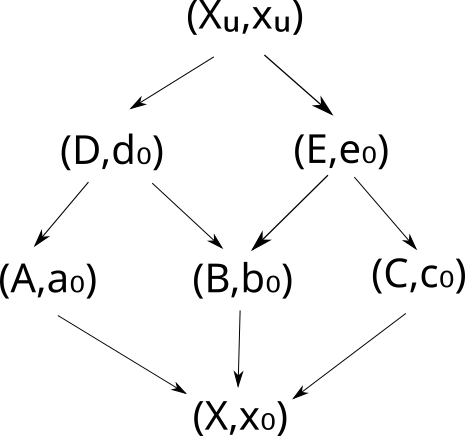
\includegraphics[scale=0.3]{./imagenes/cov.png}
  \caption{caracterización categoria}
\end{figure}
Es claramente un lattice con \((X_u, x_u)\) el cubrimiento universal
como elemento inicial.

Podemos volver a definir un functor
\[ \pi : \mathscr{Cov} (X, x_0) \to \mathscr{Grp} \]
reutilizando la notación \(\pi\) para asignar a cada espacio cubrimiento
su grupo fundamental. Es claro que por ser \((X_u, x_u)\) simplemente
conexo, se cumple que
\[ \pi (X_u, x_u) = {e} \]
Mas aun, por el teorema \ref{thm:inyec-covering} de inyectividad de del
homomorfismo inducido por un cubrimiento \(p\), el lattice de
cubrimientos es respetado como estructura en la categoría
\(\mathscr{Grp}\). Por tanto el functor \(\pi\) preserva elementos
iniciales entre categorías.